\documentclass{article}

\usepackage[francais]{babel}
\usepackage[T1]{fontenc}
\usepackage{fancyhdr}       % header & footer

\usepackage{wrapfig}
\usepackage{graphicx}
\usepackage{geometry}
\geometry{hmargin=2.5cm}
\usepackage{amsmath}
\usepackage{siunitx}

\usepackage{graphicx}
\usepackage{subcaption}
\usepackage{float}
\usepackage{hyperref}
\usepackage{setspace}
\usepackage{xcolor}
\usepackage{pdfpages}
\usepackage{enumitem}
\usepackage{lscape}

\title{Réseaux industriels}
\date{2020}
\author{Laura Bin}

\begin{document}
    % \pagenumbering{arabic}
    \pagenumbering{gobble}

    \pagestyle{fancy}
    \renewcommand\headrulewidth{1pt}
    \fancyhead[L]{Laura Binacchi}
    \fancyhead[C]{Réseaux industriels}
    \fancyhead[R]{\today}

    \section*{Implémentation de la RFC echo}
    \begin{enumerate}
        \item Réaliser deux clients TCP et UDP pour le protocole echo (\href{http://tools.ietf.org/html/rfc862}{RFC 862}). Ce client se connectera sur serveur dont l'adresse sera donnée en paramètre sous forme d'URL via le port 7. Le client enverra la chaîne de caractères passée en second argument au serveur. Le client affichera ensuite la chaîne de caractères renvoyée par le serveur (la même normalement !).
        \item Réaliser deux serveurs TCP et UDP pour le protocole echo. Tester ce serveur avec le client précédent.
    \end{enumerate}

    \paragraph{Note :} un seul client et un seul serveur implémentent les deux protocoles. Pour lancer les programmes avec le protocole udp, il suffit de rajouter l'argument "udp".

    \subsection*{Protocole TCP}
    \textbf{Serveur :}
    \begin{figure}[H]
        \centering
        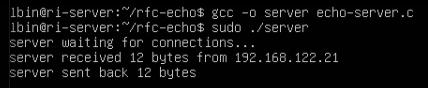
\includegraphics[width=.65\linewidth]{./screenshots/echo-server-tcp.png}
    \end{figure}

    \textbf{Client :}
    \begin{figure}[H]
        \centering
        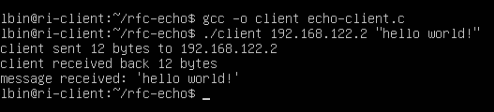
\includegraphics[width=.65\linewidth]{./screenshots/echo-client-tcp.png}
    \end{figure}

    \subsection*{Protocole UPD}
    \textbf{Serveur :}
    \begin{figure}[H]
        \centering
        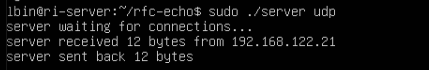
\includegraphics[width=.65\linewidth]{./screenshots/echo-server-udp.png}
    \end{figure}

    \textbf{Client :}
    \begin{figure}[H]
        \centering
        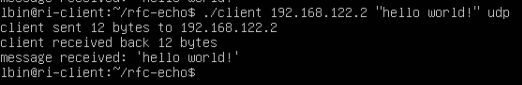
\includegraphics[width=.65\linewidth]{./screenshots/echo-client-udp.png}
    \end{figure}

\end{document}